\documentclass{article}

\usepackage{amsmath}
\usepackage{natbib}
\usepackage{graphicx}
\usepackage{siunitx}
\usepackage{float}
\usepackage{hyperref}
\newcommand\tab[1][1cm]{\hspace*{#1}}
\date{} 
\begin{document}





\begin{figure}[!tp]
\vspace{-10mm}

\includegraphics[scale=0.8]{ee.png}


\vfil
\hfil \Large \bf MIDDLE EAST TECHNICAL UNIVERSITY
 \hfil
\vfil

\vspace{5mm}
\vfil
\hfil \large \bf  EE464- STATIC POWER CONVERSION-II
 \hfil
\vfil

\vspace{5mm}
\vfil
\hfil \large \bf HARDWARE PROJECT FINAL REPORT \hfil
\vfil
\bf

\vspace{23mm}
Mert ZEYBEK    \tab\tab 2167682


Hamza SOLAK \tab\tab2263762


\vspace{5mm}
\small Date: 24/06/2020


\end{figure}

\newpage
\tab\tab
\section*{Introduction}
\tab In this project, we aimed to design a regulated and isolated DC-DC power supply using Forward Converter topology. This report contains detailed simulation results of our Forward Converter design, PCB design and 3D view of this design, component selection, bill of materials of component selection and thermal equivalent circuit of our design is provided. Basic circuitry and specifications of the Forward Converter is given below:
\begin{figure}[h]
    \centering
    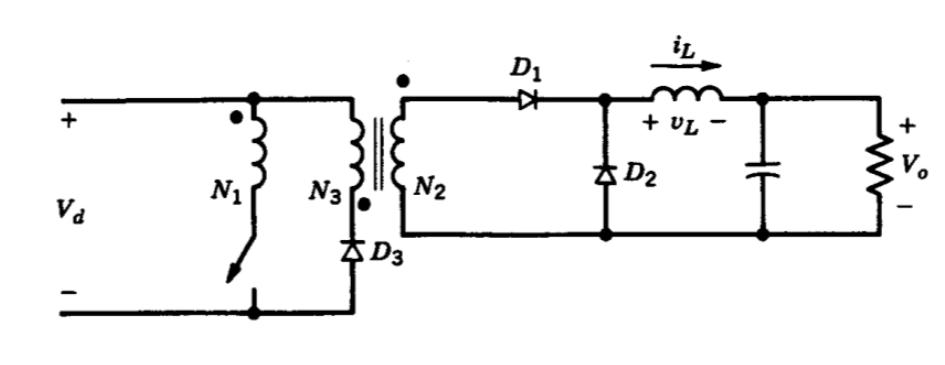
\includegraphics[scale=0.5]{forwardconverter.PNG}
    \caption{Forward converter circuit schematic }
    \label{fig:my_label}
\end{figure}

\begin{center}
Table 1: Project Design Specifications of Forward Converter
\newline \\

 \begin{tabular}{||c c||} 
 \hline
 Minimum Input Voltage & 12V \\ 
 \hline
 Maximum Input Voltage & 24V  \\
 \hline
 Output Voltage & 10V  \\
 \hline
 Output Power & 48 W  \\
 \hline
 Output Voltage Peak to Peak Ripple & 2 \% \\
 \hline
  Line Regulation & 2 \% \\
 \hline
  Load Regulation & 2 \% \\
 \hline
 \end{tabular}
 \end{center} \\
 
 \tab Considering that using Forward Converter topology instead of Flyback Converter increases cost, we aimed to come up with a more efficient converter instead of cheaper converter since using this topology already increases cost and it may not be possible to offer cheapest solution to the customers. Minimizing volume also was not our primary concern since the topology has transformer which makes its volume larger than non-isolated converter topologies such as Buck converter, Cuk converter.
 
\newpage
\section*{Design Decisions}
\tab Since we aim to make our circuit as efficient as possible, some of the design decisions that we took in the Simulation Report are revised. We tried to make core loss and copper loss of magnetizing elements as close as possible since we assume it is the ideal and most efficient case. Semiconductor devices are also revised to minimize losses on them. Output capacitor is also replaced with several parallel capacitors so that we can minimize ESR value.
\subsection*{1) Magnetic Design}
\tab\textbf{a) Transformer Design} \\
\tab Firstly, we selected our switching frequency. We selected it as 10 kHz. Although it is relatively small value for that kind of application, it decreases losses which is our main goal. Then we calculated our desired area product for the transformer considering our design specifications as follows, where $P_{out}$ is output power, J is current density, K is topology constant, $B_{max}$ is maximum flux density and f is frequency:

 \begin{equation*}
     W_aA_c=\frac{P_{out}J}{K B_{max} f}=\frac{48*500}{0.0005*1300*10*10^3}=3.69 cm^4
 \end{equation*}
 \tab Since we desire to have a high permeability core for Forward Converter, ferrite cores fit better for our application. Considering these, \href{https://www.mag-inc.com/Media/Magnetics/Datasheets/0P44022EC.pdf}{0P44022EC} is selected. It is an E shaped, P material type ferrite core, whose area product is $4.59 cm^4$. Its geometric shape is given below:
 \begin{figure}[H]
    \centering
    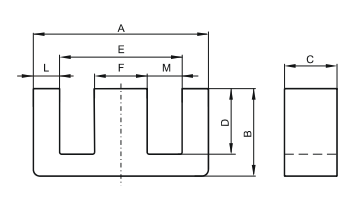
\includegraphics[scale=0.5]{transformer.PNG}
    \caption{Geometric Shape of Transformer Core}
    \label{fig:my_label}
\end{figure}
 \tab After that, we calculated our required primary number of turns for the transformer as follows:
 \begin{equation*}
    n_1>\frac{V_i_{max}*D_{max}}{f_s*B_{sat}*A_e}=\frac{24*0.5}{10^4*0.3*0.000233}=17.167
\end{equation*}
$n_1$ is selected as 18. Considering we always need to stay below 0.5 duty cycle so that we do not saturate the core and considering additional voltage losses in realistic simulation, we calculated $n_3$ $ \frac{n_3}{n_1}=1.2$. As a result, $n_3$ is selected as 22. $n_2$ is selected as 18 as well, equal to $n_1$. After that, appropriate cable sizes are selected for each winding for current density of $4 A/mm^2$. Maximum input current is assumed to be 2.08 A and output current is assumed to be 5 A considering power and voltage ratings. As a result, AWG18 for primary side, AWG14 for secondary side and AWG25 for reset winding is selected. Fill factor is calculated to whether we can fit these cables inside the core or not as follows:
\begin{equation*}
    k_f=\frac{A_{cable}}{A_e}=\frac{((18*0.82+22*2.08+18*0.16) mm^2}{233 mm^2}=0.272
\end{equation*}
Fill factor is relatively small, on the other hand it shows that cables can fit into the core and having a large core can help us reduce core losses. \\
\tab Copper losses are calculated with selected cable sizes. To do that, mean length per turn value was necessary, which is calculated as below for E shaped transformer:
\begin{equation*}
    MLT=\frac{ \pi*(E-F)}{4}= 13.59 mm
\end{equation*}

After that, primary and secondary winding resistances are found as follows:

\begin{equation*}
    R_{1}=20.9428*18*13.59*10^{-6}=5.123 mOhms
\end{equation*}

\begin{equation*}
    R_{3}=8.282*22*13.59*10^{-6}=2.476 mOhms
\end{equation*}

Using $I^2R$ formula, copper loss is calculated as follows:
\begin{equation*}
    P_{copper}=I_1^2R_1+I_3^2R_3=2.08^2*5.123*10^{-3}+5^2*2.476*10^{-3}=84 mW
\end{equation*}

\tab To calculate core loss, Steinmetz's Equation is used. It is specified as follows:
\begin{equation*}
    P_{CL}=\frac{a*f^x*B^y*L(T)}{1000} mW/cm^3
\end{equation*}
\tab To use this equation, a, x and y constants, which are material specific, are needed. For P type material Magnetics provided these values as $a=3.2$, $x=1.46$ and $y=2.75$. L(T) is also a function of ambient temperature and it is given as $1$ for $100 Celcius$ temperature. It is assumed to be 1 in the calculation:
\begin{equation*}
     P_{CL}=\frac{3.2*(10*10^3)^{1.46}*0.3^2.75}{1000}=137.91 mW/cm^3
\end{equation*}
Multipliying it with $V_e$ of the core which is $5590 mm^3$, we can find $P_{core}$ as follows:

\begin{equation*}
   P_{core}=P_{CL}*V_e=137.91*22.7=3.13 W
\end{equation*}
\tab\textbf{b) Inductor Design}
\newline \tab At inductor design, we want to limit output current ripple which would also ensure continuous conduction mode. We want to keep the converter in CCM since forward converter's gain changes a lot in DCM. On the other hand, choosing a too large inductor would increase DCR value, which would reduce efficiency. We considered following equations for calculation of our output inductor considering 2 \% ripple rating:
\begin{equation*}
    I_{L_O,min}=I_{O,max}*0.02 =4.8*0.02=0.096 A
\end{equation*}
Ripple value must be less than twice of this value which is given below:
\begin{equation*}
{\displaystyle \Delta }I_{L_o}=(\frac{n_3}{n_1}*V_i-V_o)*\frac{1}{L_o}*t_{on}<0.192 A
\end{equation*}
\tab As a result, we need an inductor with $3.8 mH$ inductance in order to meet criteria. This value is relatively high since our switching frequency is small. As a result, we needed to select a core with high inductance per turn square value. Using \href{https://www.mag-inc.com/getattachment/Products/Ferrite-Cores/Learn-More-about-Ferrite-Cores/Magnetics-Ferrite-Catalog-2017.pdf?lang=en-US}{this} catalog of Magnetics, \href{https://www.mag-inc.com/Media/Magnetics/Datasheets/0W44715TC.pdf}{0W44715TC} is selected as our inductor core. Its geometric shape is given below:
\begin{figure}[H]
    \centering
    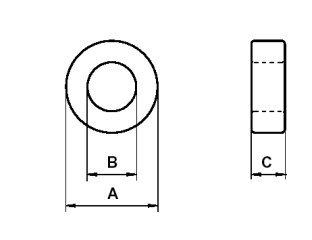
\includegraphics[scale=0.4]{inductor.PNG}
    \caption{Geometric Shape of Inductor Core}
    \label{fig:my_label}
\end{figure}
Its $A_L$ value is defined as $16100 nH/T^2$ at 10 kHz, which is our switching frequency. Number of turns is calculated as follows:
\begin{equation*}
    N=10^3*\sqrt\frac{L}{A_L}=10^3*\sqrt\frac{3.8 mH}{16100 nH}=15.36 \approx 16 turns
\end{equation*}
Assuming it will carry more or less same amount of current with the secondary winding of the transformer, we can choose AWG14 cable for inductor as well.Fill factor according to these selection is calculated below:
\begin{equation*}
    K_f=\frac{A_{cond}}{W_a}=\frac{2.08*16}{145}=0.230
\end{equation*}
After that, length of cable that is going to used for inductor is necessary to determine copper loss on the inductor. 

\begin{equation*}
    MLT=(A-B)+2C=49.9 mm
\end{equation*}

\begin{equation*}
    P_{copper}=I^2R=4.8^2*8.282*16*49.9*10^{-6}=317 mW
\end{equation*}
\tab To find core losses, Steinmetz's Equation is used once more.  According to that, core loss is calculated below:
\begin{equation*}
    P_{core}=V_e*a*B^b*f^c=16.063*10^{-3}*31.320*0.3^{1.585}*40^1.371=44.26 mW
\end{equation*}
\subsection*{2) Closed Loop Control}
\tab Since we desire to have a constant output voltage with variable input voltage, we need to have a closed loop controller. To do that, we used TL494 integrated circuit. Its pin output is given below:

\begin{figure}[H]
    \centering
    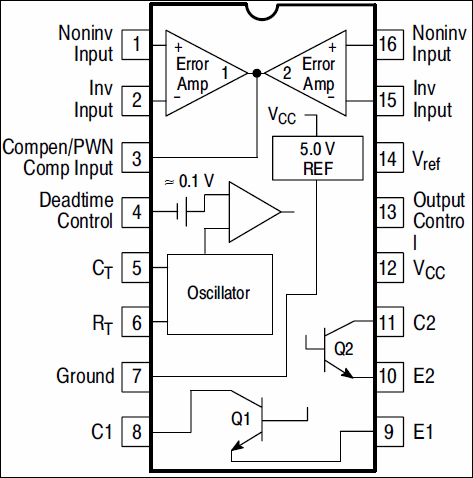
\includegraphics[scale=0.2]{tl494.png}
    \caption{TL494 Pin Output Diagram}
    \label{fig:my_label}
\end{figure}

\tab First thing to do while deciding our parameters was setting oscillation frequency equal to our selected switching frequency, which is 10 kHz. $R_T$ and $C_T$ values are calculated according to the following formula:

\begin{equation*}
    f_s=\frac{1}{R_TC_T}
\end{equation*}
$C_T$ is selected as 1 nF and $R_T$ is selected as 100 kOhms.  \\
After that, we moved to Error Amplifier circuit in order to keep output voltage constant, whose schematic is given below:

\begin{figure}[H]
    \centering
    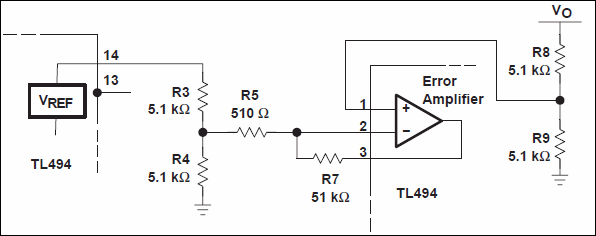
\includegraphics[scale=0.5]{error.png}
    \caption{TL494 Error Amplifier Circuit}
    \label{fig:my_label}
\end{figure}

\tab In this circuitry, $R_3$ and $R_4$ resistances create a reference voltage of 2.5 V. $R_8$ and $R_9$ enables us to sample our output voltage and $R_5$ and $R_7$ determines the gain of the amplifier. We decided to stick to resistance values that were given in the example circuit given above, since they meet our requirements. From the TL494 schematic, we can see that there are two error amplifiers in this circuit. However, the other amplifier is usually used for current limiting, which we do not want to have in this case. As a result, we decided to connect its positive input to supply voltage and negative input to ground, so that we never limit the current. \\

\tab After that, we moved on to soft start future of TL494, which can be helpful in limiting stresses on the devices by avoiding high starting currents. Soft start circuit of TL494 is given below:

\begin{figure}[H]
    \centering
    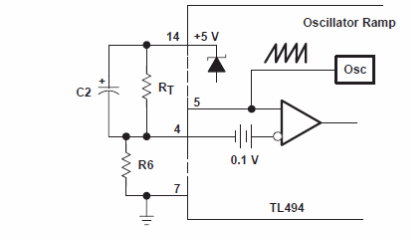
\includegraphics[scale=0.5]{soft.PNG}
    \caption{TL494 Soft Start Circuit}
    \label{fig:my_label}
\end{figure}

\tab Soft start time is selected as 15 ms, which is 150 cycles period for 10 kHz frequency. According to that, $C_2$ is selected as 3.3 uF AND $R_6$ is selected as 4.7 kOhms. \\

\tab TL494 is good at creating the PWM signal that we desire. However, it cannot drive a MOSFET directly with its output signal. Considering this, we decided to use an TLP250 digital optocoupler. It also creates isolation between high voltage part and low voltage part of the circuit, which is another advantage. TLP250 circuit is given below:

\begin{figure}[H]
    \centering
    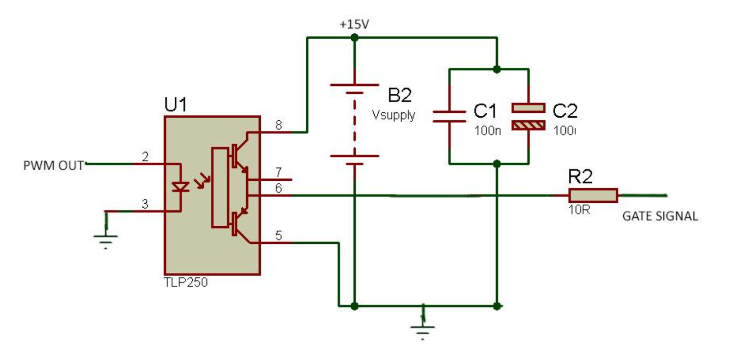
\includegraphics[scale=0.5]{opto.PNG}
    \caption{TLP250 Digital Optocoupler Circuit}
    \label{fig:my_label}
\end{figure}
\tab We needed an another optocoupler in order to isolate output from the controller circuit. We decided to use HCNR200 for this purpose. Its pin diagram and circuitry are given below:
\begin{figure}[H]
    \centering
    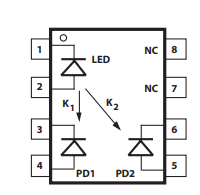
\includegraphics[scale=0.8]{analog opto.PNG}
    \caption{HCNR200 Analog Optocoupler Pin Diagram}
    \label{fig:my_label}
\end{figure}

\begin{figure}[H]
    \centering
    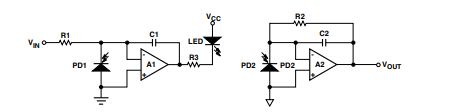
\includegraphics[scale=1]{analog opto devre.PNG}
    \caption{HCNR200 Analog Optocoupler Isolation Circuit}
    \label{fig:my_label}
\end{figure}

\tab Lastly, we need a buck converter to supply integrated circuits that we used in controller without using an external supply. For that, we decided to use D36V6F15 regulator, whose output voltage is 15V and input voltage can be between 50 V-15.2 V, which covers our input range. Its picture is given below:
\begin{figure}[H]
    \centering
    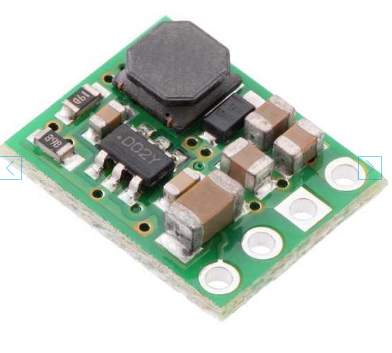
\includegraphics[scale=0.3]{buck.PNG}
    \caption{D36V6F15 Regulator}
    \label{fig:my_label}
\end{figure}

\end{document}